\documentclass[letterpaper,twocolumn]{article}

% Math packages
\usepackage{amsthm}
\usepackage{amsmath}
\usepackage{amssymb}

% For more complicated table formatting
\usepackage{multirow}
\usepackage{tabularx}
\newcolumntype{L}[1]{>{\raggedright\let\newline\\\arraybackslash\hspace{0pt}}m{#1}}
\newcolumntype{C}[1]{>{\centering\let\newline\\\arraybackslash\hspace{0pt}}m{#1}}
\newcolumntype{R}[1]{>{\raggedleft\let\newline\\\arraybackslash\hspace{0pt}}m{#1}}

% Remove line spaces between items of enumerate and itemize
\usepackage{enumitem}
\setlist{noitemsep}

% Adds double bracket symbols
\usepackage{stmaryrd}

% Allows to create negation symbols
\usepackage{MnSymbol}

% General math symbols
\DeclareMathOperator{\Id}{Id} % Identity function

% Theorem styles

%\renewcommand\thesubsection{\thesection.\Alph{subsection}}
%\renewcommand{\theequation}{\thechapter.\arabic{equation}}

\newtheorem{assump}{Assumption}
\renewcommand*{\theassump}{\Roman{assump}}

\newtheorem{axiom}[equation]{Axiom}
\newtheorem{defn}[equation]{Definition}
\newtheorem{prop}[equation]{Proposition}
\newtheorem{coro}[equation]{Corollary}
\newtheorem{thrm}[equation]{Theorem}

%\theoremstyle{definition}

\newenvironment{remark}{\emph{Remark}.}{}
\newenvironment{rationale}{\emph{Rationale}.}{\qed}
\newenvironment{justification}{\emph{Justification}.}{\qed}
\renewenvironment{proof}{\emph{Proof}.}{\qed}


% LOGIC symbols
% -------------

% Boolean symbols and algebra
\def\Bool{\mathbb{B}}
\def\TRUE{\textsc{true}}
\def\FALSE{\textsc{false}}
\def\AND{\wedge}
\def\bigAND{\bigwedge}
\def\OR{\vee}
\def\bigOR{\bigvee}
\def\NOT{\neg}

% Logical context and related symbols
\def\logCtx{\mathcal{S}}
\def\vstmtSet{\mathcal{S}_\textsf{v}}
\def\dstmtSet{\mathcal{S}_\textsf{d}}
\newcommand{\pAss}[1][\mathcal{S}] {\mathcal{A}_{#1}}
\DeclareMathOperator{\truth}{truth}

% Experimental test symbols
\newcommand{\exptSet}{\mathcal{E}}
\newcommand{\expt}[1][e] {\mathsf{#1}}
\DeclareMathOperator{\result}{result}
\def\SUCCESS{\textsc{success}}
\def\FAILURE{\textsc{failure}}
\def\UNDEF{\textsc{undefined}}

% Statements
\def\tautology{\top} % Tautology
\def\contradiction{\bot} % Contradiction
\newcommand{\stmt}[1][s] {\mathsf{#1}} % Statement
\newcommand{\tstmt}[1][s] {\bar{\mathsf{#1}}} % Theoretical statement

% Relationships between statements
\def\comp{\doublefrown} % Compatibility
\def\ncomp{\ndoublefrown} 
\def\narrower{\preccurlyeq} % Narrowness
\def\nnarrower{\npreccurlyeq}
\def\snarrower{\prec}
\def\nsnarrower{\nprec}
\def\broader{\succcurlyeq} % Broadness
\def\nbroader{\nsucccurlyeq}
\def\sbroader{\succ}
\def\nsbroader{\nsucc}
\def\indep{\upmodels} % Independent
\def\nindep{\nupmodels}

% Experimental domains and related symbols
\newcommand{\edomain}[1][D] {\mathcal{#1}} % Experimental domain
\newcommand{\tdomain}[1][D] {\bar{\mathcal{#1}}} % Theoretical domain
\newcommand{\basis}[1][B] {\mathcal{#1}} % Basis
\newcommand{\resPoss}[1][x] {\mathring{#1}} % Residual possibility
\newcommand{\estPoss}[1][x] {\dot{#1}} % Established possibility

% Formatting for experimental relationships
\newcommand{\erel}[1][r] {#1}

% Formatting for sentence statements
\newcommand{\statement}[1] {\emph{``#1"}}

% Formatting for reference
\newcommand{\refStmt}[1][r]{\textbf{#1}}

\DeclareMathOperator{\ver}{ver}
\DeclareMathOperator{\fal}{fal}
\DeclareMathOperator{\und}{und}

\DeclareMathOperator{\interior}{int}
\DeclareMathOperator{\exterior}{ext}

% Level of detail
\def\eqgran{\doteq}
\def\finer{\leqdot}
\def\nfiner{\nleqdot}
\def\coarser{\geqdot}
\def\sfiner{\lessdot}
\def\scoarser{\gtrdot}

\usepackage{graphicx}
\usepackage{hyperref}
\hypersetup{
	colorlinks=true,
	citecolor=blue,
	urlcolor=blue,
	linkcolor=blue
}
\urlstyle{same}
\usepackage[font=scriptsize]{caption}

\begin{document}

\title{Counting evolutions: a simple foundation for thermodynamics}
\author{Gabriele Carcassi\footnote{carcassi@umich.edu}, Christine A. Aidala, et al \\ University of Michigan}

\date{\today}

\maketitle

\begin{abstract}
	In this work we present the core ideas at the heart of a new approach to the foundations of thermodynamics. The premise is to focus on the count of evolutions: the possible ways the state of a system can evolve in time. We see that in a deterministic process the evolutions can never diverge and in a reversible one they can never merge. This means that the count of evolutions per state can never decrease under a deterministic process and it is maximized at equilibrium. We show how this simple idea can be used as a straightforward foundation of thermodyanmics and how it relates to other notions of entropy in physics.
	
	This work is part of Assumptions of Physics, a project that aims to identify a handful of physical principles from which the basic laws can be rigorously derived  (\url{https://assumptionsofphysics.org}).
\end{abstract}


\section{Introduction}

This working draft summarizes the status of our work on a new approach to the foundations of thermodynamics and is intended to gather early feedback. Rather then derive thermodynamics bottom-up from a particular microscopic model, we want to derive it top-down from a set of requirements on the dynamics of the system. The results we find are, then, independent on the microscopic dynamics in the sense that they can in principle be realized in different ways. This is both more in line with the aims of the founders of thermodynamics and justifies why thermodynamic concepts have been successful in fields beyond physics. Moreover, in our approach thermodynamics is found as a specialization of a more general model, which we believe can be used as a common foundation for the different types mechanics.

In a nutshell, we characterize processes in general terms, as the description of all possible ways that the system can evolve in time, its possible evolutions, under a particular set of circumstances, as one can see in figures \ref{fig_single_evolution} through \ref{fig_with_equilibria}. Counting the possible evolutions plays a fundamental role, in much the same way that counting states plays a role in statistical mechanics. In a deterministic and reversible process, all evolutions that start in one state will end in the same state: the evolutions cannot merge or diverge. If the process is deterministic but not reversible, however, the same final state can be reached from different initial states, and the evolution will merge. If the deterministic process reaches an equilibrium, there will be no more merging. We define process entropy to be the logarithm of the count of evolutions per state, which we find to have the basic properties we associate with entropy: it is linear under system composition of independent systems, can never decrease under a deterministic process, increases if the process is non-reversible and is maximized at equilibrium. This gives us a conceptually crisp physically meaningful concept that is tied to irreversibility and equilibria in a very natural way.

There are many technical details that are required to make the above characterization formally rigorous, mostly due to the proper handling of infinities. However, those do not really change the overall intuition, which we believe is the main strength of the approach. Therefore, in this paper, we will only give a conceptual overview leaving the formal details to other papers. This will leave the key physical insight is more directly accessible, and also result in a narrative that can be used directly in an introductory course of thermodynamics.

\section{States, processes and evolutions}

The first question we want to answer is: how can we characterize processes in the most general terms? We assume we have a system and we want to study its behavior in a given set of circumstances. If the state space $X$ of the system represents all possible configurations the system can be found in, ultimately we want to characterize how the state changes in time. As depicted in figure \ref{fig_single_evolution}, we have a copy of the state space at each moment in time, and we call an \textbf{evolution} a trajectory $x(t)$ that for each moment in time returns the state of the system. 

\begin{figure}[h]
	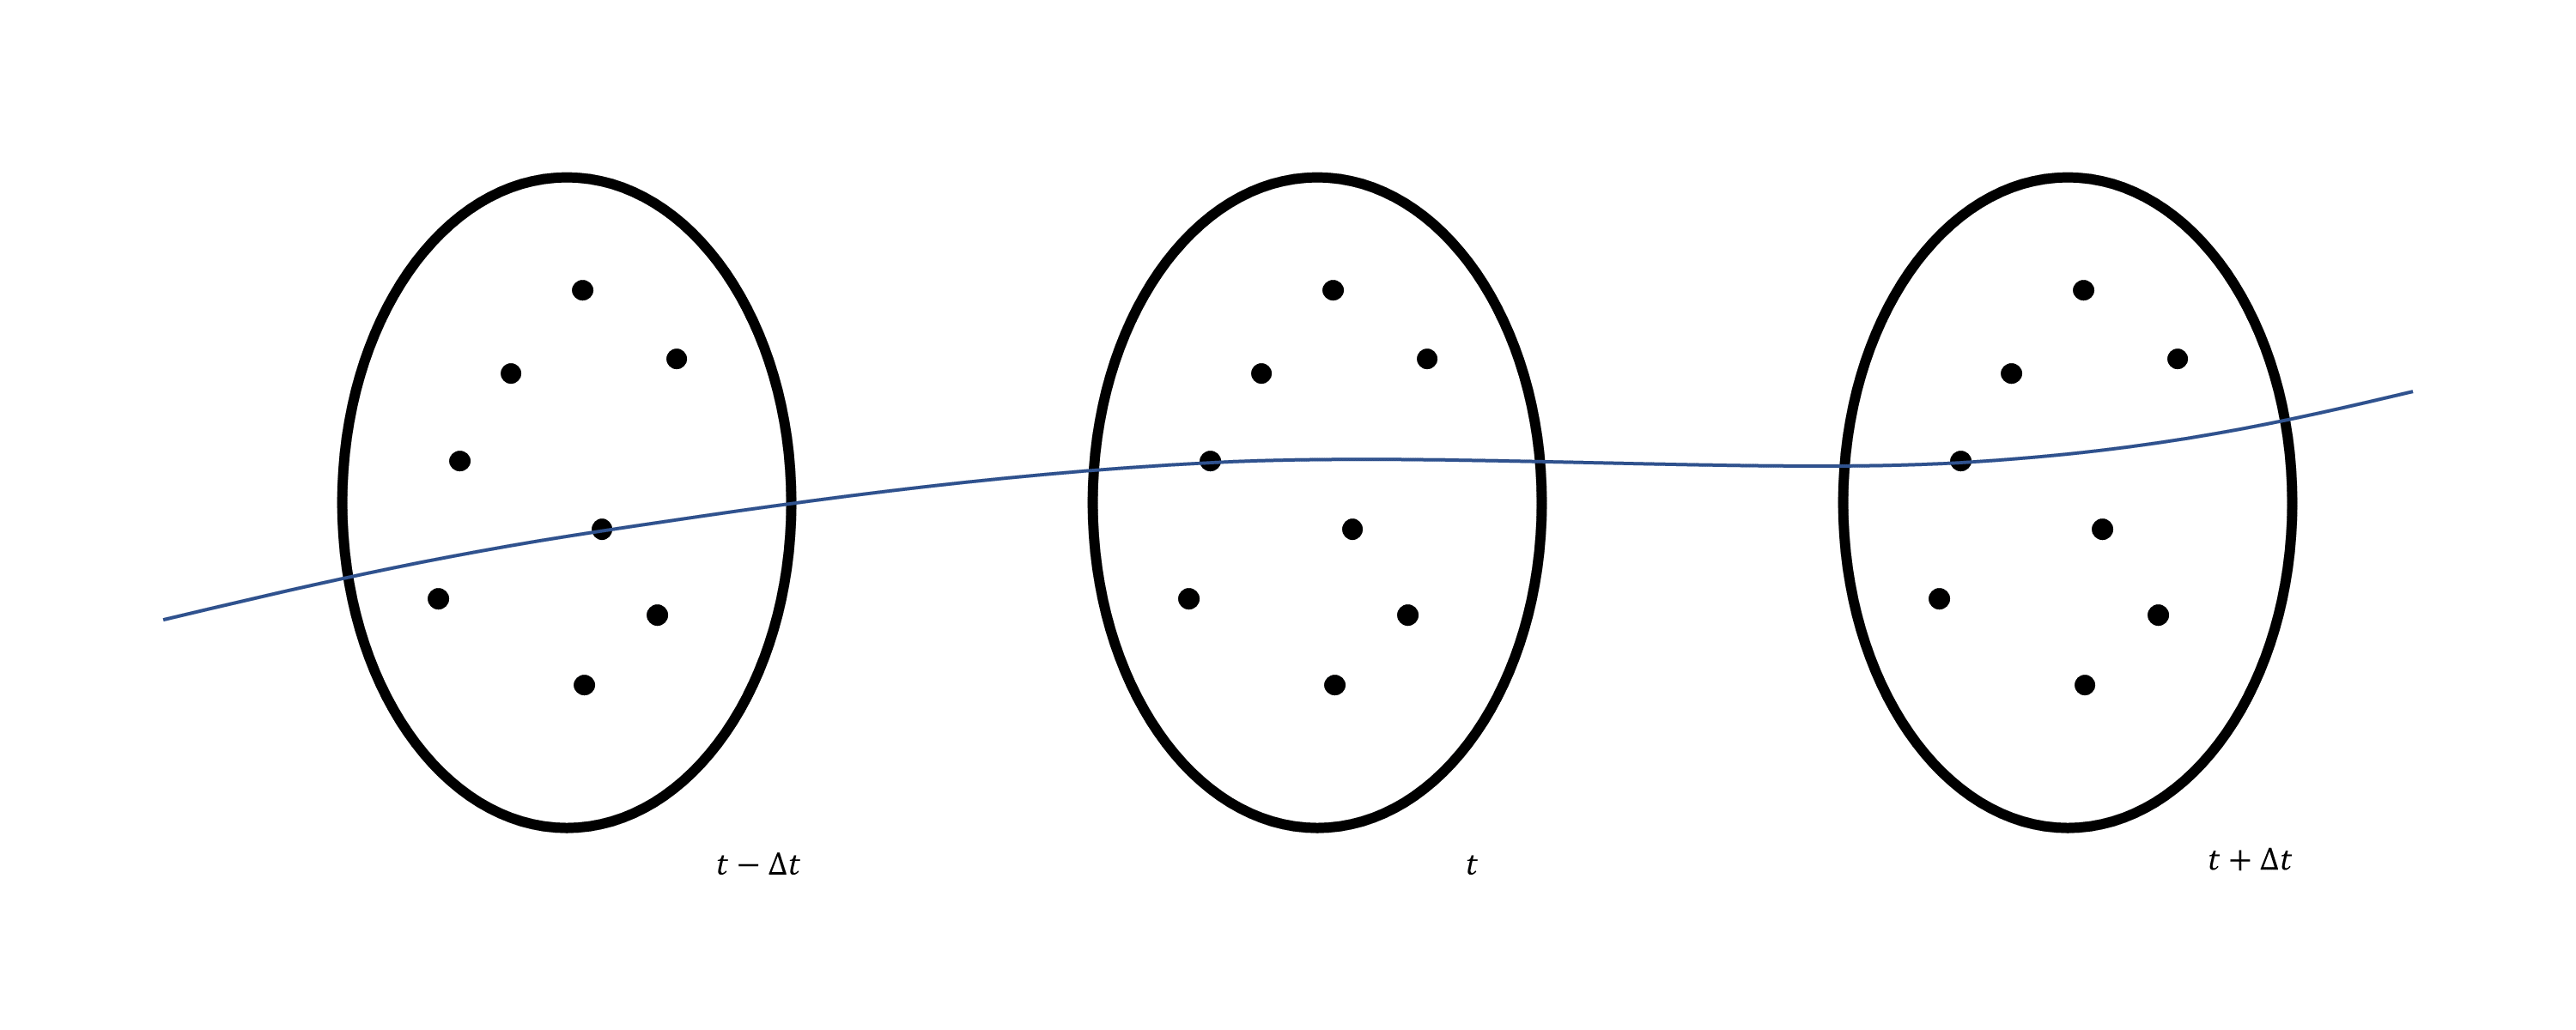
\includegraphics[width=\columnwidth]{images/Slide1.png}
	\caption{The three sets represent the state space of the same system at three different moments in time. The blue line is an evolution, which tells us the state of the system at all times.}\label{fig_single_evolution}
\end{figure}

Not all evolutions will be possible under all conditions. Therefore we choose to characterize a \textbf{process} simply as the set of allowed evolutions, as we can see in figure \ref{fig_process}. Namely, a process tells us what can and cannot happen in a given set of circumstances. We also assume we have a measure $\mu$ that allows us to determine the size of a set of evolutions, to ``count'' evolutions.\footnote{The precise conceptual and mathematical definition for $\mu$ is source of a number of technical considerations which we (will) address in a separate work. While some issues, like unit definition, are important to the physics, most have to do with the proper handling of infinities or the conditions for existence and uniqueness of the measure. Overall, they would distract from the key insights.} A state $x_t$ at a time $t$ identifies a set of of compatible evolutions $A(x_t)$, those that pass through that state at that time. That is, $x(t) = x_t$. Using $\mu$ we can give a size to that set, which we can write as $\mu(A(x_t))$ or $\mu(x_t)$ for short.

\begin{figure}[h]
	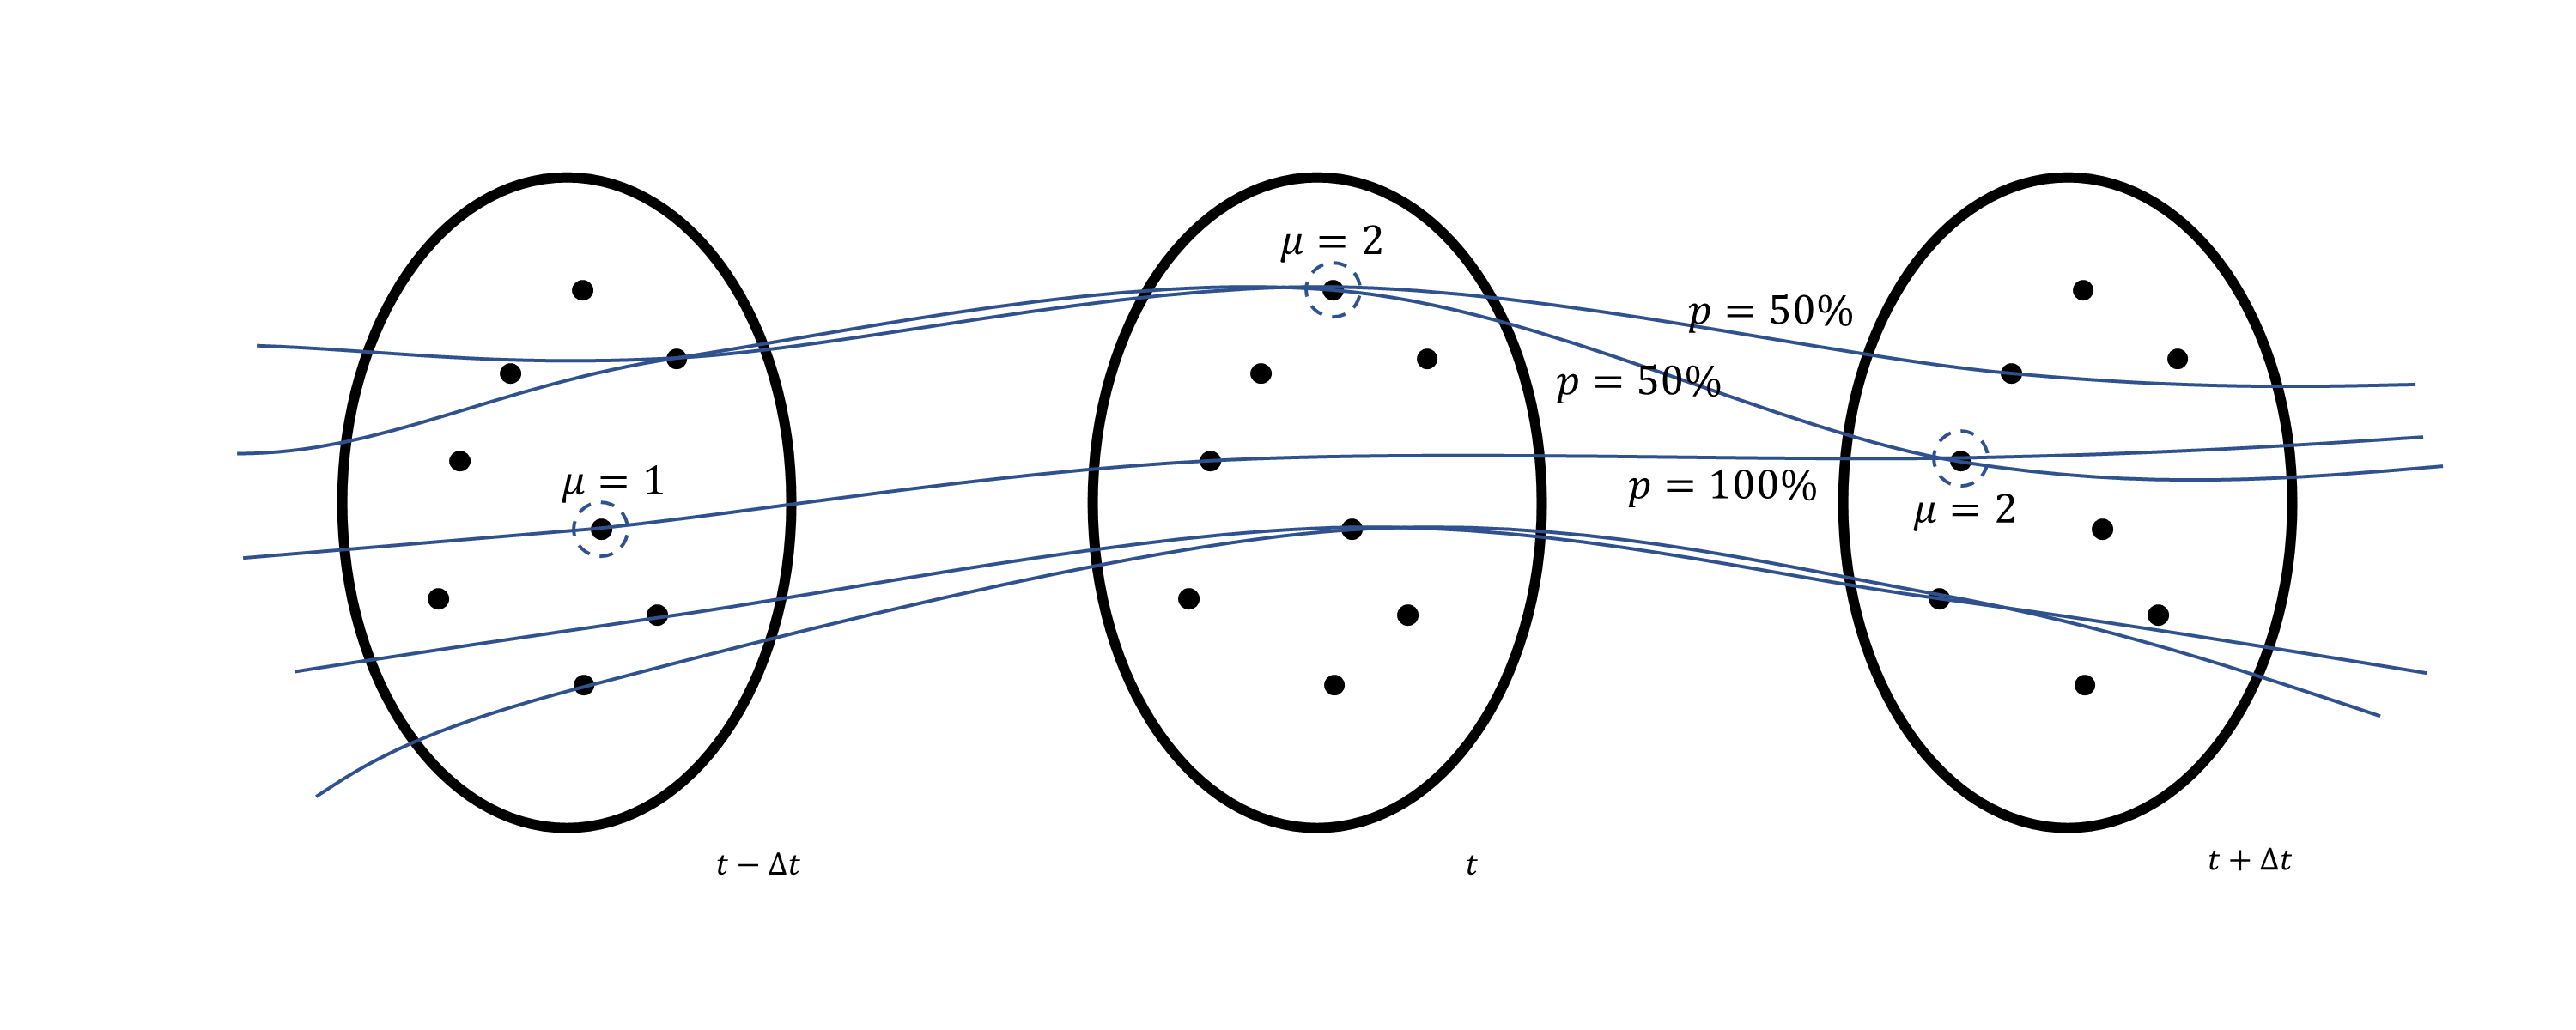
\includegraphics[width=\columnwidth]{images/Slide2.png}
	\caption{A process is characterized by the set of all possible evolutions. The measure $\mu$ allows us to express the size of a set of evolutions. The probability of transitioning from one state to another corresponds to the fraction of evolutions that starts in the first and also ends in the second.}\label{fig_process}
\end{figure}

Note that the probability of transitioning from one state to another during a process is linked to the allowed evolutions and their count. In fact, calculating the probability of finding the state $x_{t+\Delta t}$ at $t+\Delta t$ given $x_t$ at $t$ means determining the fraction of evolutions that pass through $x_t$ that also pass through $x_{t+\Delta t}$. That is:
\begin{equation}
	P(x_{t+\Delta t} | x_t) = \frac{\mu(A(x_t) \cap A(x_{t+\Delta t}))}{\mu(A(x_t))}.
\end{equation}
Conceptually, the ability to count evolutions is equivalent to knowing all possible probability of transition.\footnote{Technically, a single probability measure is not enough to define all these transition at all scales, but the overall intuition remains.}

Having answered the question of how we characterize processes, we can categorize them. For example, we say a process is \textbf{deterministic} if the state at one time in enough to determine the state at all future times. We can see an example of such a process in figure \ref{fig_determinism}. In this case, if two different evolutions happen to reach the same state at a given time, they will also share all future states: evolutions can merge but cannot diverge. The count of evolutions per state over time can never decrease: $
\mu(x(t)) \leq \mu(x(t + \Delta t))$.

Deterministic processes can be characterized by a law of evolution. That is, we can write $x(t+\Delta t) = f(x(t), t)$ given a suitable function $f$ which may, in general, be time dependent. We can do this because $P(x(t+\Delta t) | x(t)) = 0$ for all but one future state. The law of evolution identifies that state. That is, $P(x(t+\Delta t) | x(t)) = 1$ if and only if $x(t+\Delta t) = f(x(t), t)$.

\begin{figure}[h!]
	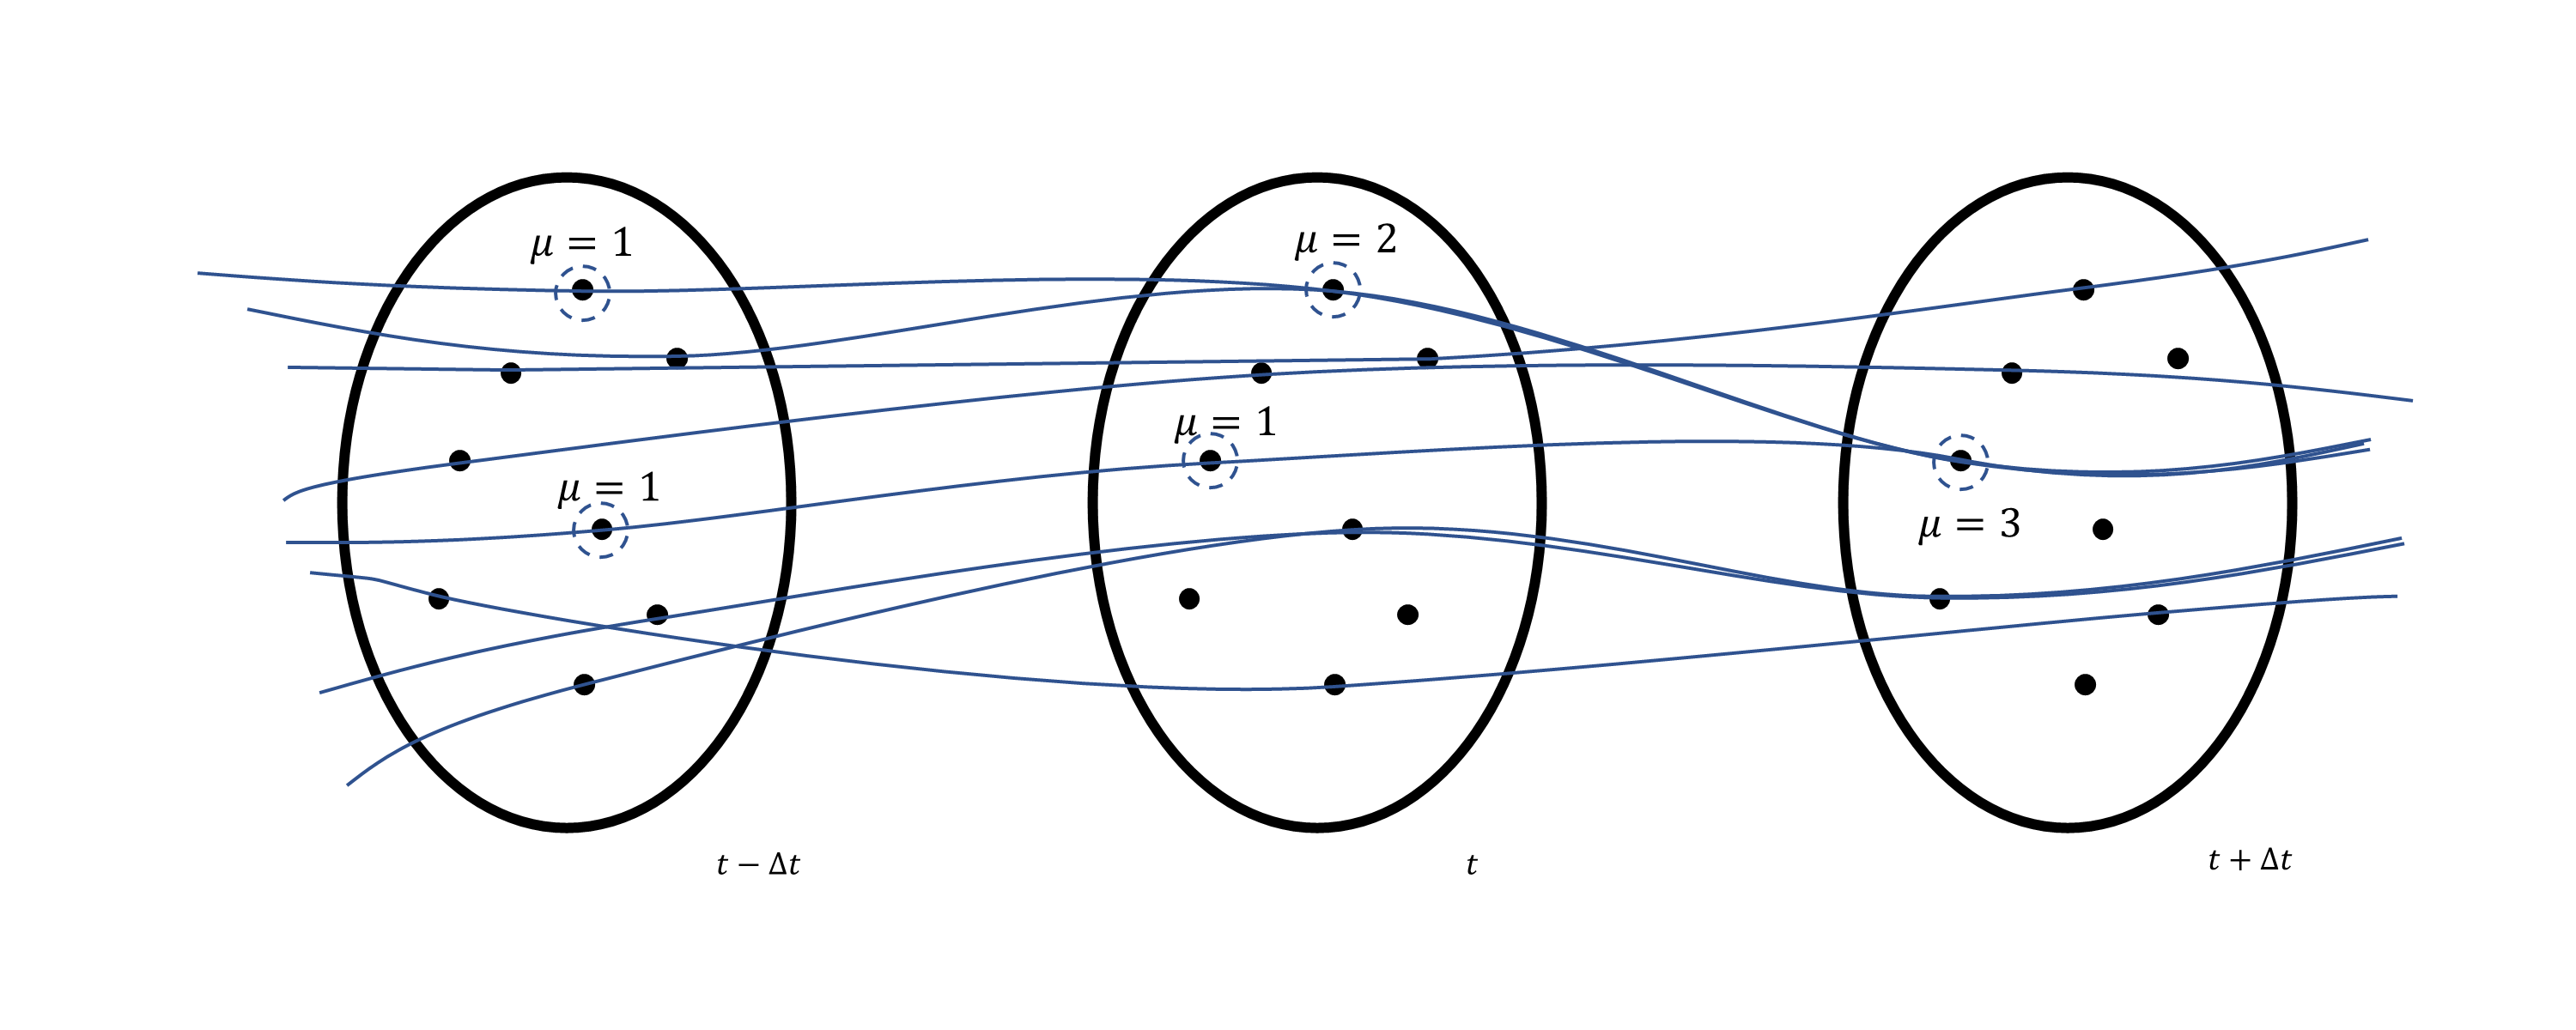
\includegraphics[width=\columnwidth]{images/Slide3.png}
	\caption{Deterministic process: the state one time determines the state at future times. Evolutions can merge but not diverge in time. The number of evolutions per state cannot decrease.}\label{fig_determinism}
\end{figure}

Conversely, we say a process is \textbf{reversible} if the state at one time is enough to reconstruct the state at all past times.\footnote{Note that in some literature the ability to reconstruct the past is called retrodictability and does not coincide with thermodynamic reversibility (the ability to undo a change). This distinction appears in the context of continuous quantities and it is precisely one of those technical considerations we (will) address in a more technical work. At this point we want to make it clear that our notion of reversibility will indeed correctly recover thermodynamic reversibility. It will do so without having to assume the existence of a reverse process or a symmetry under time-reversal.} We can see an example of such a process in figure \ref{fig_reversibility}. In this case, if two different evolutions happen to reach the same state at a given time, they will also share all past states: evolutions can diverge but cannot merge. The count of evolutions per state over time can never increase: $
\mu(x(t)) \geq \mu(x(t + \Delta t))$.

\begin{figure}[h!]
	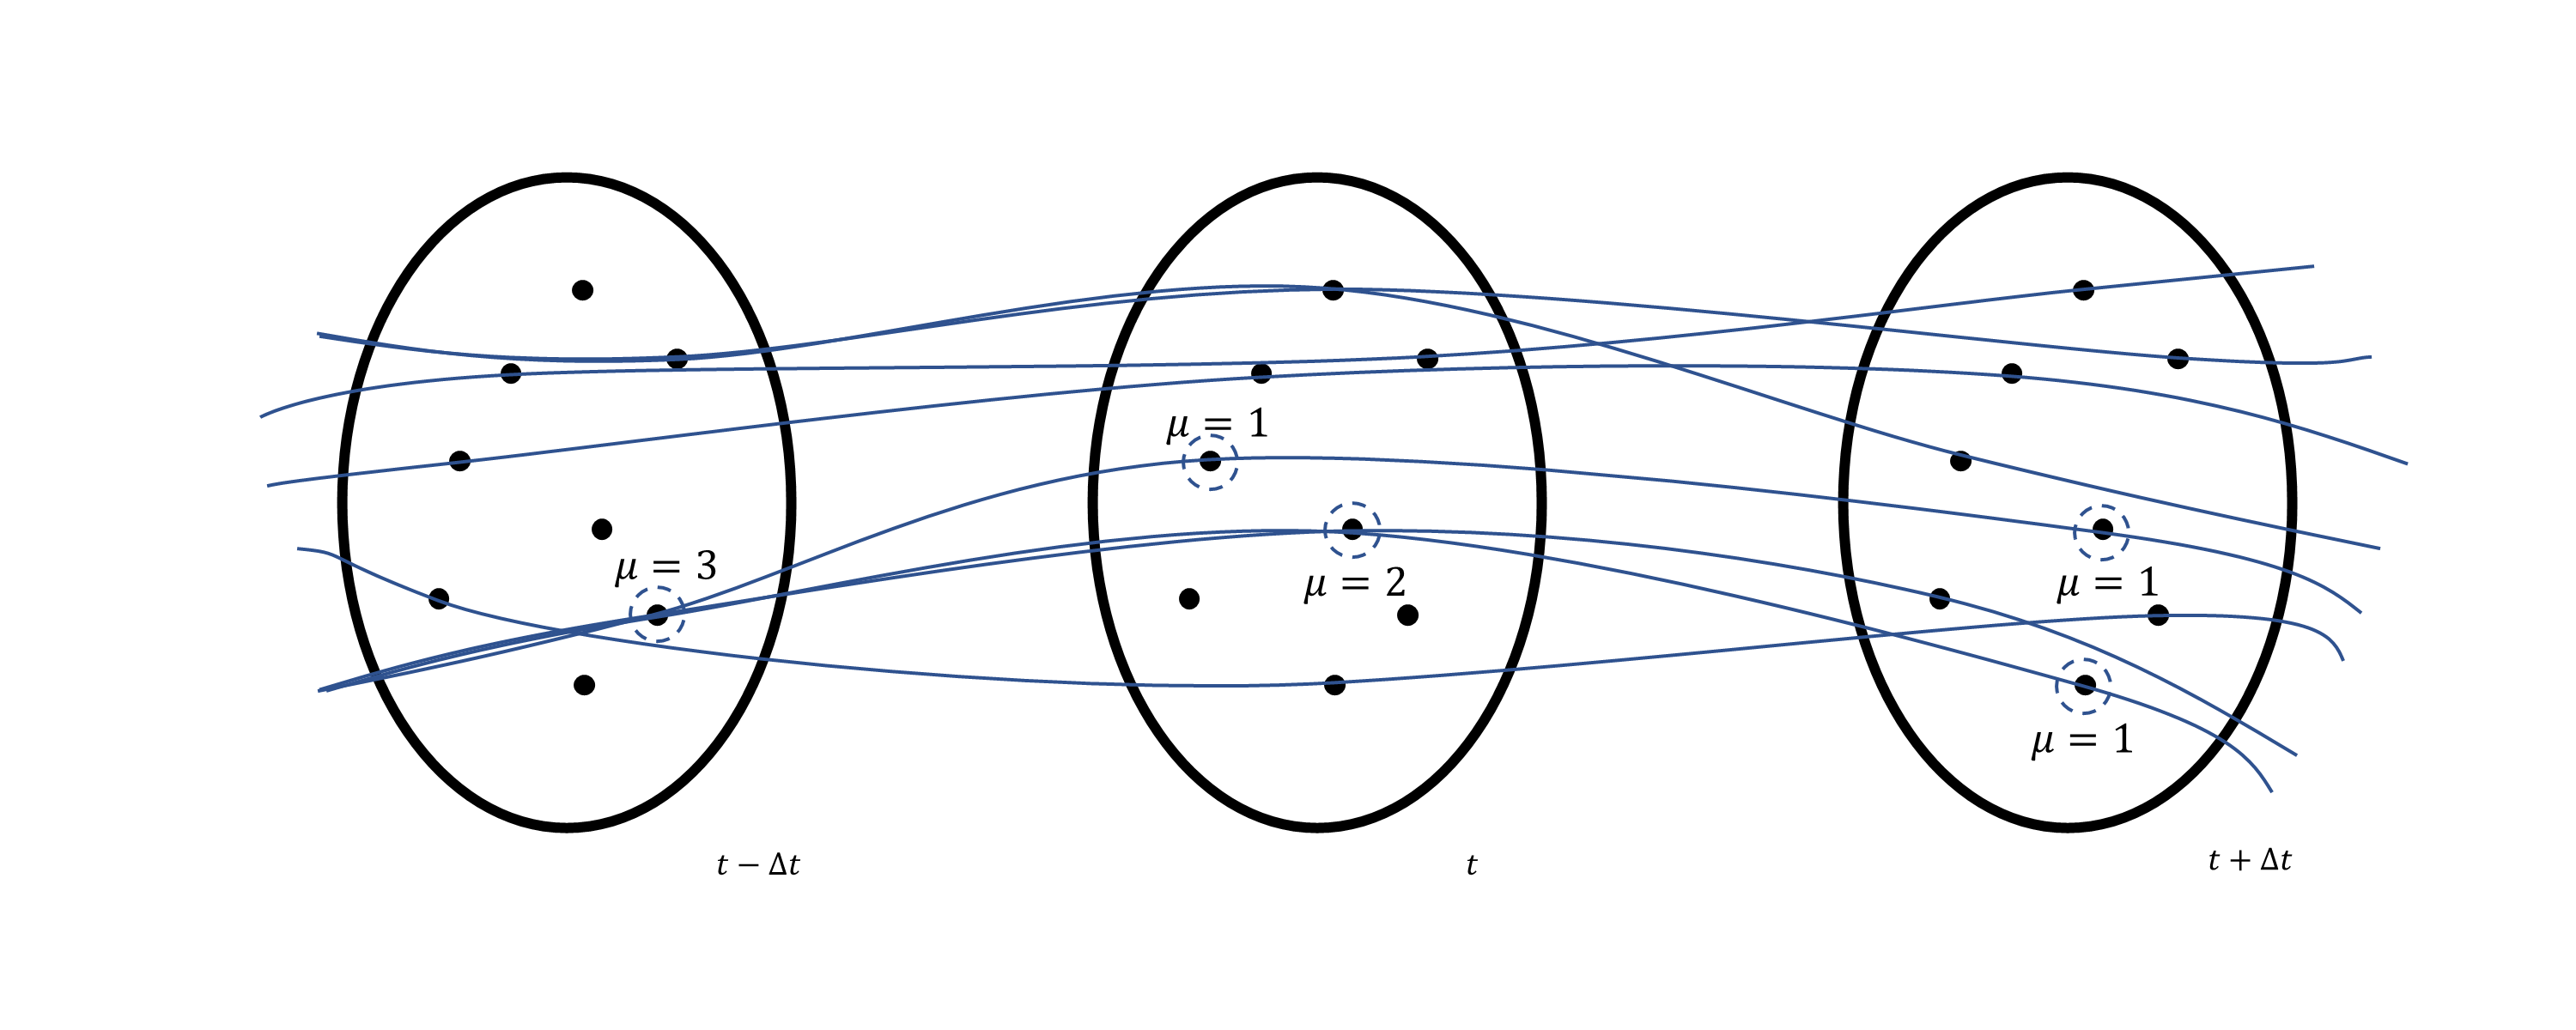
\includegraphics[width=\columnwidth]{images/Slide4.png}
	\caption{Reversible process: the state one time allows one to reconstruct the state at past times. Evolutions can diverge but not merge in time. The number of evolutions per state cannot increase.}\label{fig_reversibility}
\end{figure}



A process that is both deterministic and reversible, like the one in figure \ref{fig_detrev}, will never contain evolutions that split or merge. The count of evolutions per state over time will be a constant: $\mu(x(t)) = \mu(x(t + \Delta t))$.

%TODO: add a double evolution in some case.
\begin{figure}[h!]
	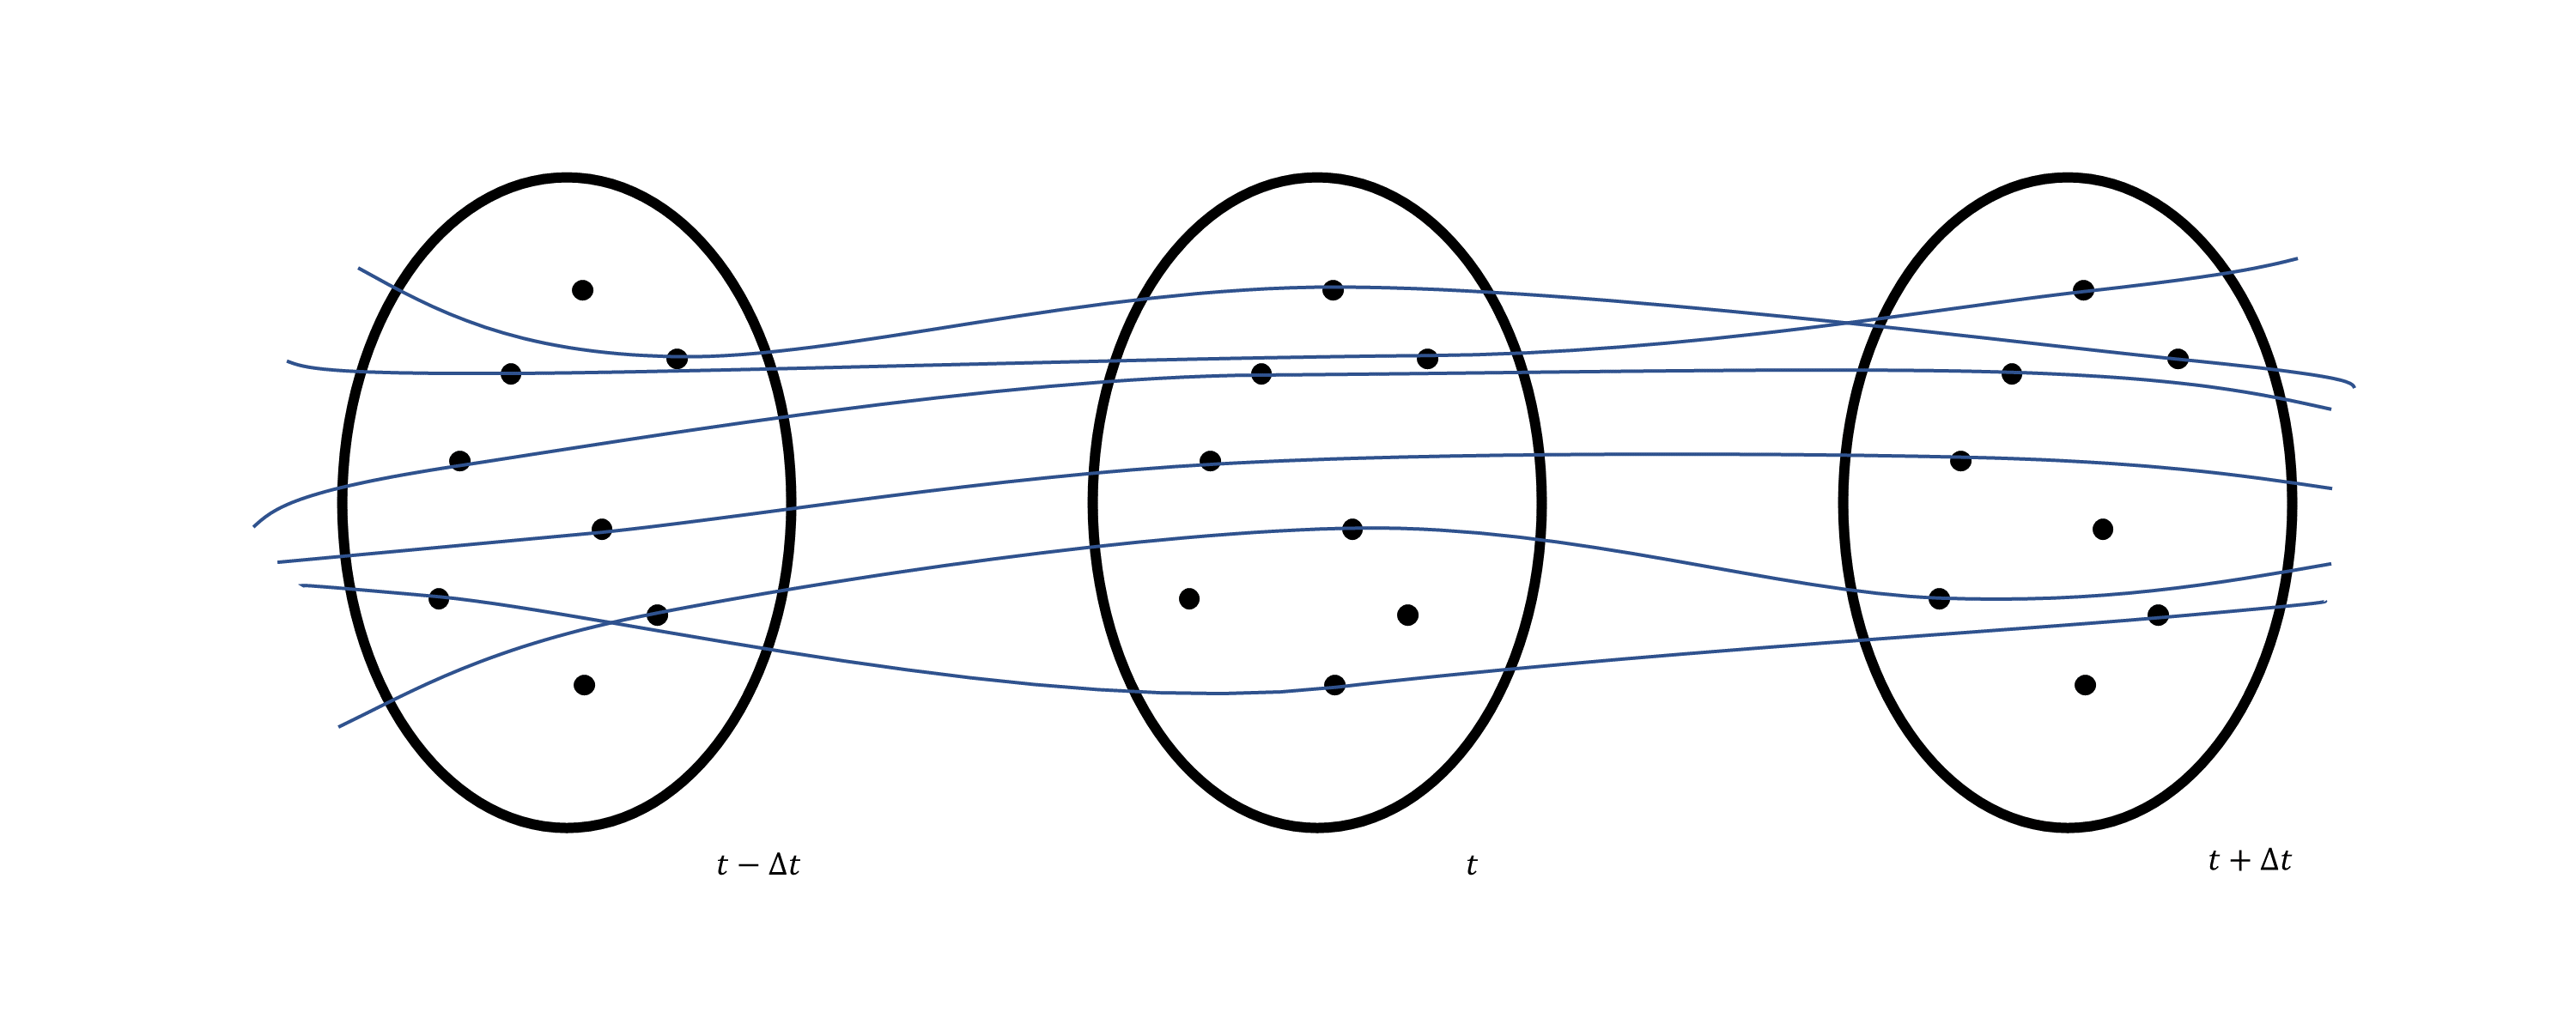
\includegraphics[width=\columnwidth]{images/Slide5.png}
	\caption{Determinism and reversibility. Evolutions cannot merge nor split. The number of evolutions per state cannot increase.} \label{fig_detrev}
\end{figure}


To finish, consider a \textbf{deterministic processes with equilibria}. We can see an example of such a process in figure \ref{fig_with_equilibria}. An equilibrium for a process is a state that, once it is reached, it is never left.\footnote{We will see later that this characterization of equilibrium is symplistic, but it will suffice for now.} In a process with equilibria all evolutions will reach, at some point, an equilibrium. In the out-of-equilibrium phase, evolutions merge until they reach equilibria and can no longer merge. This means that our measure $\mu$ is maximized at equilibria. If we care to characterize only the initial and final state, deterministic evolution simply means that the final equilibrium is a function of the initial state.

\begin{figure}[h]
	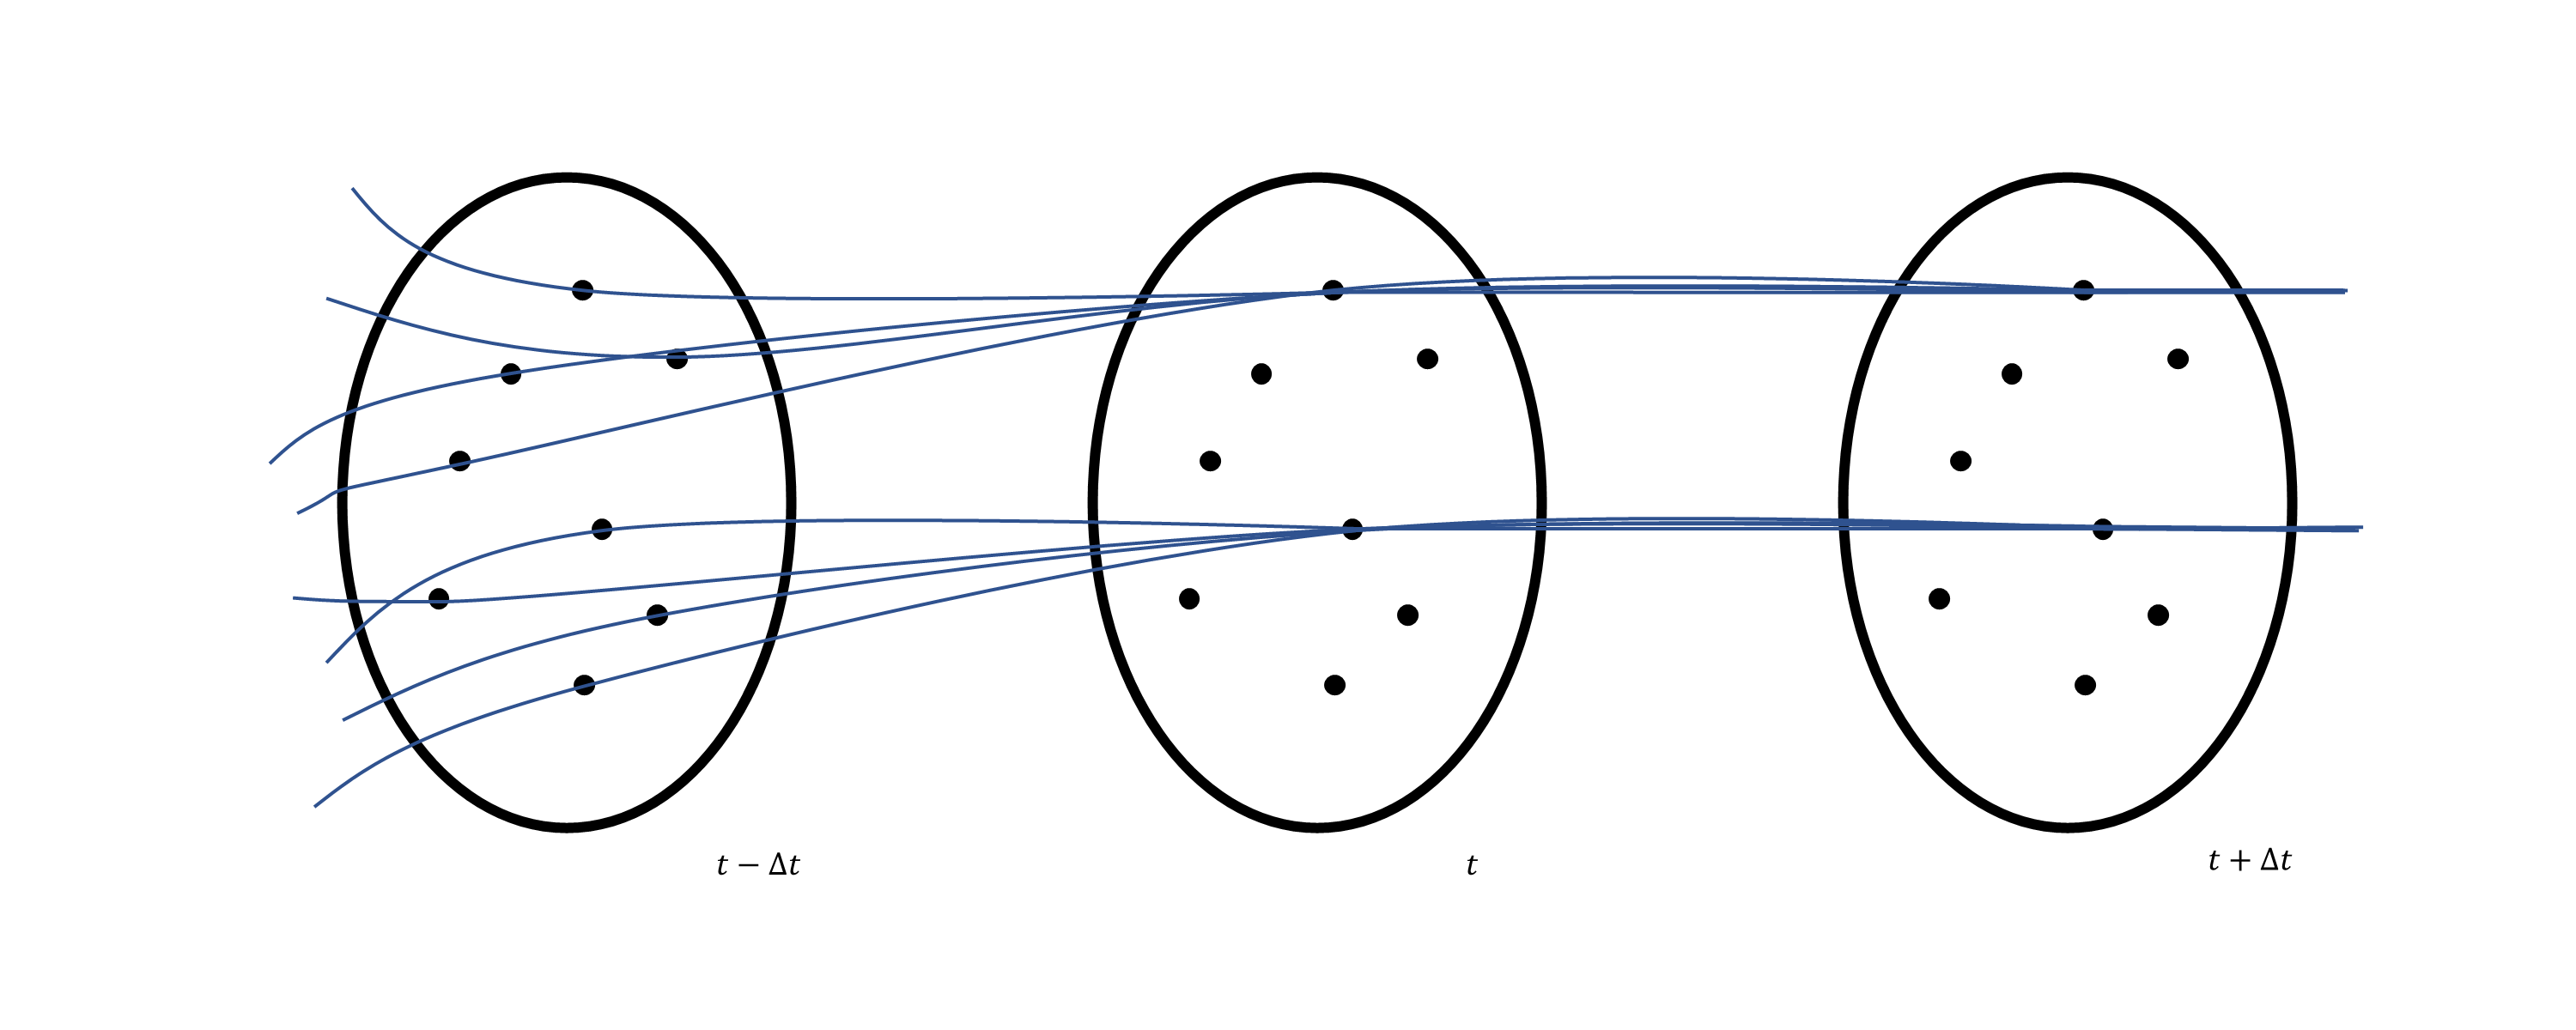
\includegraphics[width=\columnwidth]{images/Slide6.png}
	\caption{Deterministic process with equilibria. Evolutions keep merging until equilibrium is reached. The number of evolutions per state increase and the maximum is reached at equilibria.}\label{fig_with_equilibria}
\end{figure}

We already reached an important result: with only a handful of simple definitions we have found a quantity, $\mu(x(t))$, that can never decrease in a deterministic process, stays the same if the process is reversible and is maximized at equilibrium. We have done so with no assumption on the type of system, the type of forces acting on the system, the internal composition of the system or the internal dynamics of the system. It knows nothing of uncertainty, disorder, information, statistical or probability distribution, phase space volumes. It only knows about evolutions and how to count them. The result is completely general and the justification is very straight forward. It is conceptually a perfect candidate for the thermodynamic entropy, though we have one questions left: how does it combine under system composition?

Suppose we now have two systems, with their respective state space $X$ and $Y$. The state space of the composite system is the set of all possible pairs $X \times Y$. A process defined on the composite system will come with a measure $\mu_{X \times Y}$ that enables us to count evolutions $\{x(t), y(t)\}$ of the composite system. In general, the evolution of one system will affect the evolution of the other system. This will not happen, however, if the systems are independent. That is, as shown in \ref{fig_independence}, for each possible evolution $x(t)$ of the first system and $y(t)$ of the second system, there will be a possible evolution $\{x(t), y(t)\}$ on the composite. In other words,
\begin{equation}
	\mu_{X \times Y} = \mu_X \mu_Y
\end{equation}
the measure factorizes. We say two system are \textbf{independent} at given time $t$ if the evolutions per state factorizes: $\mu_{X \times Y}(x(t), y(t)) = \mu_X (x(t)) \mu_Y (y(t))$.

\begin{figure}[h]
	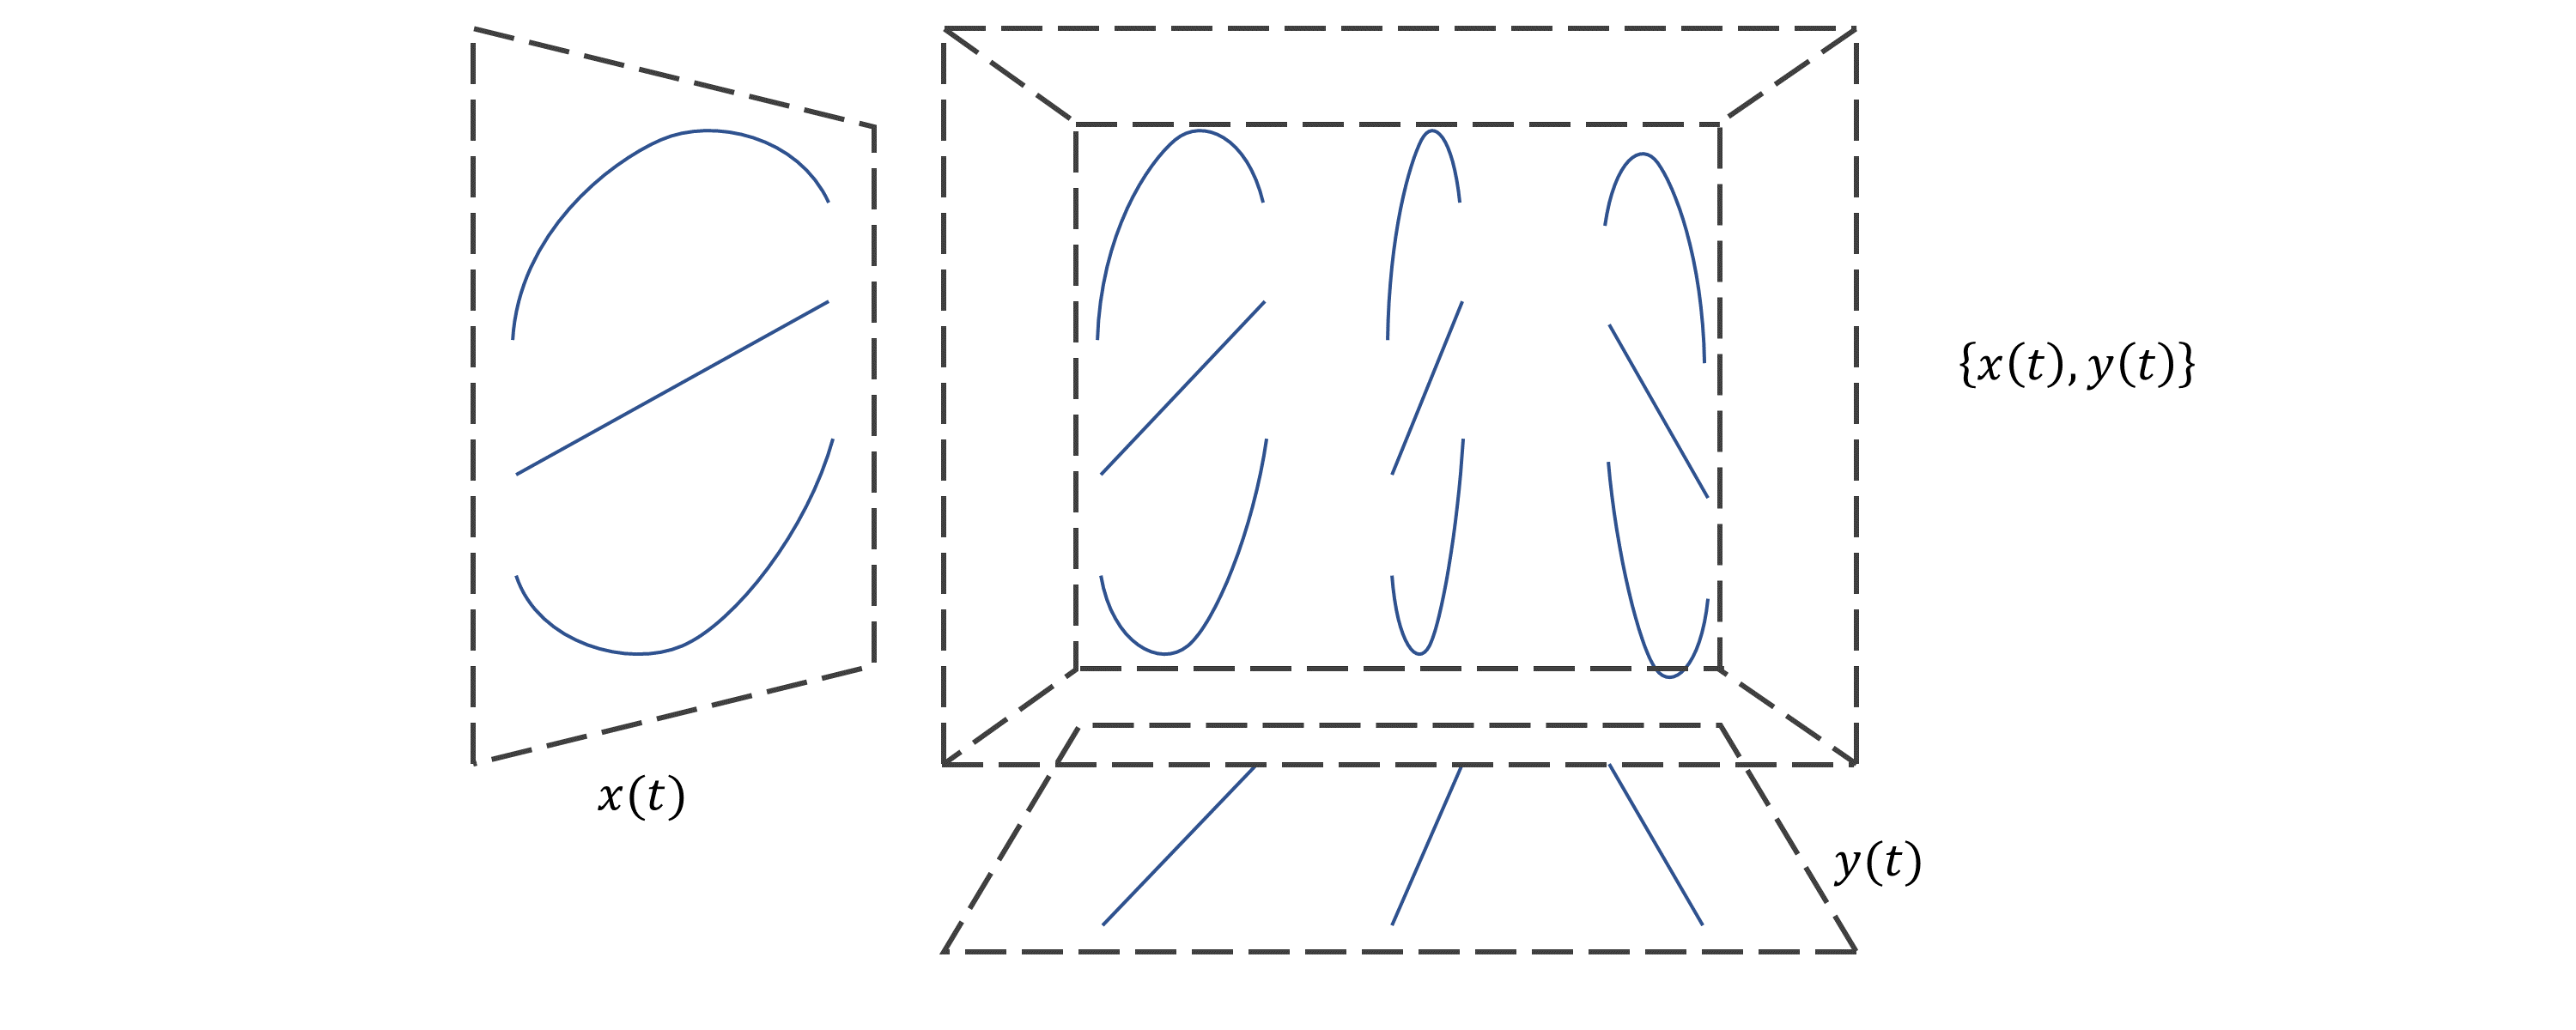
\includegraphics[width=\columnwidth]{images/Slide7.png}
	\caption{Independent system. If two systems are independent, the evolution of one does not restrict the evolution of the other: all pairs are possible. The number of evolutions factorizes.}\label{fig_independence}
\end{figure}

We define the \textbf{process entropy} as $S = \log(\mu)$. Since the logarithm is a monotonic function, the process entropy will preserve monotonicity and maximization of $\mu$ under deterministic process with equilibria. Which means:
\begin{equation}\label{ov_entropy_increases}
S(x(t)) \leq S(x(t + \Delta t))
\end{equation}
In addition, the process entropy will be additive for independent systems.\footnote{As before there are a number of technical details that need to be addressed, most of all the units for $\mu$ which will influence the 0 point for $S$. We (will) address in the full framework.}

Under very minimal conditions, we have found a quantity that has all the right properties for entropy and that is linked with determinism and irreversibility in a plain, intuitive and physically meaningful way.

\section{System independence and state entropy}

The careful reader will have noticed that the process entropy will depend on the process, not just on the state. That is, the same description of the same system may be associated with more or fewer evolutions depending on the conditions. Entropy in physics, however, is associated to a state. Under what conditions can we associate a unique process entropy to a state?

A unique value for process entropy can be assigned to states of equilibrium. Suppose, in fact, that the state $x$ is an equilibrium for two different processes $A$ and $B$. Suppose that at the end of process $A$ the system is at equilibrium $x$ and we switch to process $B$. Since $x$ is also an equilibrium for $B$, every evolution of $A$ that ended in $x$ will correspond to an evolution in $B$ that ends in $x$. By symmetry, the converse is also true. Therefore the process entropy of an equilibrium does not depend on the process, only on the equilibrium state.

If the system is a composite there are additional considerations. Different processes may put different degree of correlation between subsystems, therefore the same equilibria for the subsystems may correspond to different processes entropy values for the composite. But if the subsystems are independent, the composite will correspond to a unique entropy value: the product.

We can then assign a unique process entropy to states of equilibria and to composite state of independent equilibria. In these conditions we define the \textbf{state entropy} $S(x)$ which corresponds to the process entropy that the system reaches at equilibrium. But why would we want to assign a unique process entropy to states in the first place? Why would this be interesting? There are three main reasons.

The first is process combination. Suppose that we are studying a system and we change the circumstances surrounding it. It first evolves according to $A$ and we switch to process $B$. If $x(t)$ is an evolution of the combined process $AB$, then for $t\leq t_0$ it must be an evolution for $A$ and for $t\geq t_0$ it must be an evolution for $B$. Moreover, the number of total evolutions must remain the same. Therefore the state $x(t_0)$, the state where we are joining the evolutions, must have a well defined entropy that is independent on the process, or not all the evolutions would match. If we want to mix and match from a set of possible processes, then the process entropy at the junction must be only a function of the state.

The second reason is that, upon close inspection, measurements are never defined at a instant of time. Therefore $x(t)$, the state at an instant of time, is really a shorthand for $x[(t - dt/2, t + dt/2)]$, the state defined over a small open interval $dt$ around $t$. We can talk about a single state within that interval only if all state variables do not change and the system is fully characterized by those state variables alone. Therefore writing $x(t)$ implicitly assumes two things: that the system is an equilibrium of the processes that happen at a faster scale of our measurements of said system; that further description (e.g. the internal dynamics of the constituents at a finer scale) is not needed to describe the process.

The third reason is that by state we implicitly mean a description of a system and only about that system. If there are correlations between that system and others at a time, then the description of one will tell us more than that system alone. Proper states are then defined in the case where the system is independent, where all the correlations have been removed. This is true also for correlations with the environment and correlations between subsystems. But the condition of independence is precisely the condition that maximizes entropy, making it uniquely defined. 

All three insights points toward the same directly: the very notion of state seems to be intrinsically associated to the notion of equilibrium and state entropy. This would suggest that all states for all systems are, in a sense, equilibria. But what is exactly this sense?  What does it mean that a mechanical system, classical or quantum, is at equilibrium?

Even in thermodynamics, equilibrium is usually an ill-defined concepts. It is typically associated the one coming from dynamical systems (i.e. the system no longer changes), but this doesn't quite work. In fact, it is not even relativistically consistent. If we have a volume of gas in thermodynamic equilibrium, we would like to say it is in equilibrium for any observer, not just the one in its rest frame. A booster observer, then, would see an equilibria where the position is indeed changing. In presence of gravitational forces, this motion would not even be linear. The notion of equilibrium as ``nothing is changing'', then, is not quite right and should be amended. But how? The previous discussion would hint toward system independence, but why system independence should be an equilibrium?

The insight is that we can define something as a system only when we are able to take it apart from the rest and study it independently. Therefore we need, at least conceptually, a process that takes that something and makes it independent from the rest, decouples it, makes it autonomous. Our ability to define a system implicitly assumes the existence of such ``decoupling'' process. Note that if the system is already independent, the decoupling process does nothing: in this sense independent systems are an equilibria of a decoupling process.

This ``decoupling'' process is what maximizes entropy. If the system is truly rendered independent, then we cannot know more than the description given by the state at that particular time. We cannot know how the system came to be in that state, we cannot know anything more about the subsystems, other systems or the environment than what the state of the system strictly tell us. All possible ways that the state can be realized must be realized in a possible evolution, or we could infer something more.  When the system is independent, the states tell us the least possible information about everything else and the evolution of anything else.

The definition of a particular system, then, is conditional on the existence of particular processes: those that render the system well defined. We can talk about the motion of a ball because we are on earth at 20 Celsius. If we were on the surface of the sun, we would not be able to talk about the ball in the first place. To define a system requires us to define a boundary, which should remain the same during the process. In mathematical terms, the state space must be a symmetry (i.e. an invariant, an equilibrium) of a group (i.e. a set of transformation, a set of processes).

The full mathematical development of these concepts is left for another work, but the conceptual foundations are simple and direct. Grouping quantities into cohesive units that ``belong together'', into systems, comes with a set of practical requirements: we need a way to prepare and study them independently. This notion of ``independence equilibrium'' is what we will use as a foundation for ``thermodynamic equilibrium'', and is generalized to all systems. It is the necessary and sufficient condition to assign state entropies. In this light, entropy maximization is not a universal law of the universe, but a necessary requirement to build models. We can only study the state of objects that allow process entropy maximization. What remains is to answer one last fundamental question: is state entropy at all related to thermodynamic entropy?

\section{Thermodynamics}

The notion of equilibrium as independence is in general not sufficient to recover thermodynamic equilibrium. So, how are they related? When does the second arise?

We saw how the notion of state as independence equilibrium came naturally when considering process composition of a single system. When the process changes, we need to reconcile the count of evolution at the junction. We now want to consider the scenario of process composition of composite systems. The idea is that we want to describe the situation in which two systems come together, evolve as a composite for some time, and then proceed to evolve separately. In this case, at each juncture we have to reconcile the evolutions of both the whole and each of the part. We need to have an independence equilibrium at both levels. What we'll find is that thermodynamics studies this case. But let's proceed in order.

We say a system is in \textbf{thermodynamic equilibrium} if:
\begin{itemize}
	\item it is at equilibrium
	\item all its parts are in thermodynamic equilibrium
	\item if another system joined with a part of the system in thermodynamic equilibrium is in thermodynamic equilibrium, then the whole is in thermodynamic equilibrium.
\end{itemize}
We say two or more systems are in thermodynamic equilibrium if their composite is in thermodynamic equilibrium. A \textbf{thermodynamic process} is a process with equilibria where the final state is a thermodynamic equilibrium. We stress that we are not saying that two systems, in general, always allow for thermodynamic equilibria. However, we contend that these are the type of processes we can mix and match to create composite processes of composite systems. What we want to explore is what happens if we had such systems and process, at least to a first approximation.

To get a feel for the definition, let us rederive the fact that thermodynamic equilibrium is transitive, also known as zeroth law. Suppose system $A$ is in thermodynamic equilibrium with system $B$ and system $B$ is in thermodynamic equilibrium with system $C$. Then the composite $B \times C$ is in thermodynamic equilibrium by definition. Since $A$ is in thermodynamic equilibrium with $B$, a part of $B \times C$, it is also in thermodynamic equilibrium with $B \times C$. Therefore $A \times B \times C$ is in thermodynamic equilibrium. But $A \times C$ is a part of $A \times B \times C$, so it is in thermodynamic equilibrium. Which means $A$ is in thermodynamic equilibrium with $C$.

The characterization of thermodynamic equilibrium we give is manifestly a part-whole relationship. It extends the notion of independence equilibrium to a composite system so that the equilibrium of the whole and the equilibrium of its parts are essentially the same equilibrium. We find that clarifying this kind of part-whole relationships make for a good conceptual starting point not only for thermodynamics, but also for the other branches of physics. This should not come as a surprise as reductionism (i.e. explaining the whole through its parts) plays an important role in science.

Another important question for a part-whole relationships is: how are the state variables of the whole related to the state variables of the parts? We define a \textbf{thermodynamic system} one that follows these rules: 
\begin{itemize}
	\item states (i.e. independence equilibria) are identified by a set of extensive quantities (i.e. additive under system composition)\footnote{It may be possible that the existence of extensive quantities can be derived from the composability of thermodynamic equilibria. Note, in fact, that we typically construct measurement scales of quantities (such as energy, mass, volume, distance, ...) by preparing unit samples and then adding or dividing them. Assuming the existence of thermodynamic equilibria may enable us similar constructions without extra assumptions. (XXX: any work related to this?) Nevertheless, for this work, we consider the existence of extensive quantities an extra assumption.
	}
	\item one such quantity is called internal energy
	\item internal energy will be conserved under any deterministic process for that system.
\end{itemize}
We will denote $U$ as the internal energy and $x^i$ as the remaining extensive quantities.

For a thermodynamic system, then, the state entropy can be expressed as $S(U, x^i)$ a function of the extensive quantities. This is simply the equation of state in entropic form, which is the starting point of Gibbs formulation of thermodynamics. [CITE] We can therefore define the relationships
\begin{align}
	\beta &= \frac{\partial S}{\partial U} = \frac{1}{k_B T} \;\;\;\;\;\; - \beta X_i = \frac{\partial S}{\partial x^i}
\end{align}
where $k_B$ is Boltzmann's constant. We find:
\begin{align}
dS &= \frac{\partial S}{\partial U} dU + \frac{\partial S}{\partial x^i} dx^i \\
&= \beta dU - \beta X_i dx^i \\
dU &= k_B T dS + X_i dx^i
\end{align}
which are the usual thermodynamic relationships, except that, for us, the state entropy $S$ dimensionless..

%Under these assumptions/definitions, we can recover the laws of thermodynamics. Let $A$ and $B$ be two thermodynamic system in thermodynamic equilibrium and let $AB$ be the composite. We have:
%\begin{equation}
%\begin{aligned}
%U_{AB} &= U_A + U_B \\
%S_{AB}(U_{AB}) &= S_A(U_A) + S_B(U_B) \\
%&= \sup \{S_A(x) + S_B(y) \, | \, x+y= U_{AB}\} \\
%\frac{1}{kT_A} = \beta_A = \frac{\partial S_A}{\partial U_A} &= \frac{\partial S_B}{\partial U_B} = \beta_B = \frac{1}{kT_B}
%\end{aligned}
%\end{equation}
%which follows the standard textbooks derivations and assumes the new equilibrium is not on a boundary point. In this case, equilibrium is achieved if and only if $T_A$ and $T_B$ are equal. Since equilibria are unique, this will also tell us that all equations of states have to be concave in $U$. If $B$ is in thermal equilibrium with another system $C$ we also have $T_B$ is equal to $T_C$ and therefore $A$ and $C$ are also in thermal equilibrium. This recovers the zeroth law.
%
%There is, however, a problem. We assumed the equilibrium is not a boundary point. It could be that system $A$ reaches its lowest energy state at a finite $T_A$ while $B$ can go to lower temperatures. This would mean that $B$

A natural question, based on the previous definition, is: to what extend thermodynamic processes can change the energy and the entropy of each system? Intuitively, there are two ``orthogonal'' directions for a change of energy: constant entropy and maximal entropy change. To study these components, it is useful to consider the following special thermodynamic systems.

We say a thermodynamic system $R$ is a \textbf{thermal reservoir} if its equation of state can be sufficiently approximated by $S = \beta U = \frac{U}{k_B T}$. Internal energy is the only state variable and the only way the entropy of the system can change. We call \textbf{heat} the energy exchanged by a thermal reservoir and we note $Q = - \Delta U$ as the energy lost by the reservoir during a thermodynamic process.

We say $M$ is a \textbf{mechanical system} if the state entropy is a constant for all states. For a thermodynamic system that is also mechanical, we therefore have  $S(U, x^i) = k_M$ for all its states. A mechanical system cannot change entropy and all states can be connected through a deterministic and reversible process. We have:
\begin{equation}
\begin{aligned}
dU &= k_B T dS + X_i dx^i = X_i dx^i.
\end{aligned}
\end{equation}
The energy of the mechanical system is effectively \emph{stored} in one of the other state variables and can be later retrieved. We call \textbf{work} the energy exchanged by a mechanical system and we note $W=\Delta U$ as the energy gained by the system during a thermodynamic process.\footnote{Note that $\frac{\partial S_M}{\partial U} = 0 = \beta_M = \frac{1}{k_B T_M}$ which means the thermodynamic ``temperature'' of a mechanical system is infinite. While this ``temperature'' has little to do with thermometers, the fact that we can always transform all work into heat but not vice-versa is just a specific case of being able to move energy from higher to lower temperature.}

We can study how changes of energy and entropy are related to each other. Consider a system composed of a generic system $A$, a thermal reservoir $R$ and a mechanical system $M$. In this setting, work represents the energy exchanged at constant entropy while heat represents energy exchanged associated with entropy change.

During a thermodynamic process, because the total energy of the system must be conserved, we have:
\begin{equation}
\begin{aligned}
&\Delta U_A + \Delta U_R + \Delta U_M = 0 \\
&\Delta U_A - Q + W = 0 \\
&\Delta U_A = Q - W.
\end{aligned}
\end{equation}
This recovers the first law of thermodynamics.

We now look at the change in entropy, which during a thermodynamic process can never decrease. Keeping in mind $M$ is mechanical, we have:
\begin{equation}
\begin{aligned}
&\Delta S_A + \Delta S_R + \Delta S_M \geq 0 \\
&\Delta S_A \geq - \Delta S_R \\
&\Delta S_A \geq \int \beta_R dQ \\
&\Delta S_A \geq \int \frac{dQ}{k_B T_R}.
\end{aligned}
\end{equation}
which recovers the second law of thermodynamics. This is just a more specialized version of \eqref{ov_entropy_increases} which is valid for any deterministic process.



The third law has many equivalent formulations. [CITE] One of them states that the entropy of any system has a non-negative lower bound which is reached by the lowest energy state. If the ground state is non-degenerate, such as a perfect crystal, its entropy is equal to zero. We can easily recover it in this form.

Recall that state entropy counts the logarithm of the possible evolutions of the system at equilibrium. The lowest possible count $\mu$ of evolution is one, which is achieved if the equilibrium can be reached only by one starting condition. In this case, $S=\log(\mu)=0$. This tells us that state entropy is non-negative and therefore is bounded from below. We now have to show that all thermodynamic systems must have a lowest energy state and that it must be a local minima for entropy.

First of all, the existence of unique thermodynamic equilibria forces $S(U)$ to be strictly concave (i.e. negative second derivative). This means that, at least in some region, $S(U)$ must either be a decreasing or increasing function. But since $S$ cannot be negative, $S(U)$ cannot be defined on the whole domain. Therefore $U$ must be bounded at least from above or below. Consequently, the minimum for entropy is reached either at the lowest or highest energy state. Now we show that either all thermodynamic systems must have a lowest energy state or they must have a highest energy state. Suppose, in fact, we had two system, $A$ has no maximum energy while $B$ has no minimum energy. Since $S_A(U_A)$ is concave, it must be a monotonically increasing function of $U_A$. This means that $\beta_A$ is always positive. Conversely, $S_B(U_B)$ must be monotonically decreasing, which means $\beta_B$ is always negative. If we put the two system in contact, the energy of $B$ will keep decreasing and the energy of $A$ will keep increasing and no equilibrium will ever be reached. Therefore all thermodynamic systems either have a minimum or a maximum energy. At this point the difference is a sign convention, so we can assume all thermodynamic systems have a minimum energy.

To finish, we note that a perfect crystalline structure fits the case where the system has only one possible evolution, so it is a zero entropy state. If there is degeneracy, there are different ways the equilibrium can be realized, there are different evolutions that will correspond to the same equilibrium which means the entropy will be greater than zero. This recovers the third law.

The laws of thermodynamics have been recovered, and we have done so only by characterizing how equilibria and state variables behave under system combination. Apart from that, we have made no assumptions on what type of system, the type of forces acting on the system, the internal composition of the system or the internal dynamics of the system. No reference to statistical mechanics or quantum mechanics is needed: the theory stands on its own. This fits the original spirit of the thermodynamics, which was to find a set of laws that would be independent on the ultimate dynamics of the constituents. Additionally, the concepts we used are directly related to the physical explanation, which is not recovered after pages and pages of calculation. The combination of these features makes this approach directly useful, for example, in an introductory physics course: a coherent self-contained explanation can be given in terms of simple definitions.

% \subsubsection{XXX Null states and thermodynamic zero}

% * Use null state as thermodynamic zero.
% * Must have zero entropy.
% * All extensive quantities for the null state must be zero.
% * Extensive quantities can be zero for a propert state (i.e. number of particle of a particular species).
% * Intensive quantities are derivative: they also have an absolute zero.
% * All extensive quantities must be non-negative?

% Sample text

%Zero entropy is usually associated to a non-degenerate ground state and the lower bound on energy is usually thought as a consequence of quantum mechanics. We saw how, in our framework, these requirements stem from the definitions. In fact, we can repeat the argument and find that \emph{all} extensive quantities. We also note that, while one typically focuses on temperature and entropy having an absolute scale, other thermodynamics variable, such as volume and pressure, have a well defined zero. Is there a better way to frame these issues? We believe there is.

%System composition $\times$ is a closed operation (i.e. given any two systems returns another system) that is commutative (i.e. $A \times B = B \times A$) and associative (i.e. $A \times (B \times C) = (A \times B) \times C$). Mathematically it makes sense to ask whether it has an identity (i.e. $A \times 0 = 0 \times A = A$), which we note as $0$ since the operation is commutative (i.e. additive). In fact, while the state space of the composite is the product of the subsystems, system composition in terms of systems is better thought of as an addition: we are putting things together. The identity, then, is naturally the ``null'' system: the empty system. We can keep adding nothing, and the system is unchanged. This makes system composition a commutative monoid, but not a group since there is no ``inverse'' system: the one that combined with the original gives us nothing.\footnote{Note that particles/anti-particle annihilation leaves something: the energy. So the ``anti''-system is not the ``inverse'' system.}

%The null system has only one possible configuration, which we call the null state, so it can only have one possible evolution. The null state of a null system is inherently in equilibrium and the state entropy is zero. In fact, the values for all extensive quantities must be zero since composing the null system with another null system still gives us a null system. Therefore, for example, $U_0 + U_0 = U_0$.

% The intensive quantities are defined as derivatives, which means their zero is also absolute: is the case where changing the extensive quantity leads to no change in entropy. This means that, in thermodynamic, all quantities must be absolute, not only temperature or entropy is absolute, but this tells us that all thermodynamic quantities must be absolute. Volume, pressure, number of particles, we already think of them as having a well defined zero.

%Some confusion comes from energy. In mechanics energy in the form of the Hamiltonian does not have an absolute zero, an arbitrary constant can be added with no ill effect. But rescaling internal energy by a constant $\hat{U}$ would make it no longer an extensive quantities: $(U_A + \hat{U}) + (U_B + \hat{U}) = U_{AB} + 2 \hat{U} \neq U_{AB} + \hat{U}$.\footnote{XXX: someone must have already said this} Now the question is whether

\section{Connections to mechanics}

While recovering thermodynamics from straight forward physical definitions has its own merits, we believe the approach can be used to offer gave additional insights new insights on classical mechanics, quantum mechanics and statistical mechanics. So we want to conclude with a few remarks on the subject that give a feel for how we intend to extend the work in the fully developed framework.

We have argued the states of a system are implicitly independence equilibria and have an associated state entropy. One does not typically speak in these terms for classical and quantum states. Is this warranted and useful? Do all mechanical system match our requirement to have constant entropy? If one looks closely, these facts are implicit assumed. For quantum mechanics, in fact, the Von Neumann entropy of every pure state is zero. In classical mechanics, a uniform measure is used to count the accessible states; additionally the Gibbs entropy is invariant under translations in phase space. It is also embedded directly in the corresponding mechanics. In both theories, given two states, we can always (at least mathematically) find a deterministic and reversible evolution (i.e. a Hamiltonian evolution or a unitary evolution) that connects the two. So the idea that mechanical systems are associated with a constant entropy, though seldom explicit, can be already deduced from the currently established theories.

Another natural question is: how does the process entropy relates to the fundamental postulate of statistical mechanics, that entropy is the logarithm of the count of states?
Suppose we give the description of a system at a given time (e.g. the energy of the system is within a particular bound). This will identify a set of possible evolutions and therefore a value for the process entropy. Also, this is the sum (or integral) of the process entropy associated with each state not ruled out by that description: every evolution will have to go through one of those states at that time. Now suppose the system is, at that time, independent from the other. Then the process entropy for each state is the state entropy, so the process entropy for that description is the sum (or integral) of the state entropy. Additionally, suppose the system is mechanical, then the process entropy for the description is, up to a constant, the count of states. Entropy as the count of microstates is easily recovered. Yet, it is recovered under specific conditions.

These conditions can be met in different scenarios. We could have an independent mechanical system under a deterministic and reversible process. Then counting evolution is the same as counting states, up to a constant, at any moment in time. In another scenario, the process is not deterministic and reversible but is isoentropic, meaning that the process entropy is constant in time. If we have an independent mechanical system, its evolution will necessarily be isoentropic since, whatever state we evolve to, the state entropy will always be the same. Now suppose the set of states compatible with our description mix with each other and only with each other. Each evolution will change state in time, but it will never go outside of the set, so the description works both as a constraint and a description of the dynamic equilibrium. At each time, the same description will correspond to the same states, so the process entropy will be constantly given by the count of states.

Then one may ask: how are these two entropies different? Imagine that the mechanical system starts independent but the dynamics is non-reversible leading the dynamical system to an equilibrium, as in a damped harmonic oscillator. The process entropy at the initial state will coincide with the count of states, but not at later times. As the evolution concentrate around the equilibrium, the number of states become fewer so the number of evolutions per state increases. The entropy of the equilibrium, assuming that it is ever reached, is essentially the size of the basin of attraction at the initial time. The entropy around the equilibrium, then, increases in time which is consistent with the process being irreversible. Conversely, note that the areas in phase space shrink as the available states become fewer and fewer, which would mean entropy as the log of the state count decreases under an irreversible process. It was actually this paradox that pushed into considering evolutions as more fundamental than states and, retrospectively, it is the obvious choice.

This example also show how critical is the notion of independence to define state entropy. The evolution of a damped harmonic oscillator is not independent from the evolution of the systems that are absorbing the dissipated energy, which are in fact correlated: the higher the energy of the oscillator, the higher the energy lost. The same description at different times (e.g. the system has reached equilibrium) does not provide exactly the same information on the system or other systems. In these cases, the state entropy does not allow us to compare apples to apples while the process entropy always does.

Having seen how the process entropy relates to the count of states, one may naturally ask: how does it compare with the Gibbs/Shannon entropy? Suppose you cannot distinguish the dynamics of a system under a given time resolution. That is, in principle the system has a well defined trajectory $x(t)$ but you can only measure quantities of the form $A[x(t)] = \int_{t_0}^{t_0 + \Delta t} a(x) dt$ (e.g. average energy, average number of particles, ...). A permutation of states within the trajectory will not affect any of the measurement outcomes. Therefore the best we can do, given enough of those measurements, is to measure the frequency $\rho(x)$ each state is visited within the time resolution. Now we ask, given a specific distribution $\rho(x)$, how many possible evolutions $x(t)$ would that correspond to? That means counting the number of permutations $W[\rho]$ we can construct. The process entropy will be $\log W$. The Shannon/Gibbs entropy is the limit of that expression if we take $x(t)$ to be continuous.

The approach, then, is not simply a nicer retelling of thermodynamics, but it can help us better understand the fundamental connection between all these theories. We stress that we are not arguing that all other notions of entropy should be abandoned in favor of process entropy: quite the contrary. Specific tools are often more useful than general tools precisely because they take advantage of the specific nature of the problem. The point is that if we are more aware of the interplay between the general definition and the more specific one we will not use the latter inappropriately.

\section{Conclusion and further work}

In this paper we gave a conceptual overview for a new approach to recover thermodynamics based on the simple idea of counting evolutions, the possible ways a system can evolve under a process. We saw that the logarithm of evolution count under a deterministic process has all the properties we associate with entropy and can serve as a foundations for thermodynamics but also as a common foundations for the other physical theories.

Our aim is to fully develop a formal framework based on these ideas, which will give us a general theory for states and processes. Conceptually, we start with all that can be observed at all moments of time; organize them into systems/degrees of freedom by grouping those that ``go together'' in the sense that they can be studied, at least under some circumstances, independently from the rest; define state spaces as ``templates'' of those descriptions that can be instantiated over time. This will force us to spell out the hidden assumptions one always have when defining systems, states and processes. The goal is to then recover the different physical theories with additional assumptions on the system or on the processes being studied.

Mathematically, we will build on our work on the logic of experimental verifiability, that already gives us the basic building blocks (i.e. topologies, $\sigma$-algebras). This need to be extended to allow us to count possibilities in general and evolutions in particular. Technically, we need a unified tool that generalizes notions of measure theory, geometry, probability and information theory as these cover specific aspect that do not work in the general case.

It is important to us that these additional efforts, while making the mathematics more precise, will not obscure the physical motivation and intuitive understanding of the framework. Mathematical consistency is a tool We believe there is a way 

These additional efforts will not change the nature of the insights presented. 

\bibliography{bibliography}


\end{document}